\documentclass{article}
% if you need to pass options to natbib, use, e.g.:
%     \PassOptionsToPackage{numbers, compress}{natbib}
% before loading neurips_2020

% ready for submission
% \usepackage{neurips_2020}

% to compile a preprint version, e.g., for submission to arXiv, add add the
% [preprint] option:
%     \usepackage[preprint]{neurips_2020}

% to compile a camera-ready version, add the [final] option, e.g.:
%     \usepackage[final]{neurips_2020}

% to avoid loading the natbib package, add option nonatbib:
\usepackage[preprint]{neurips_2020}
\usepackage[utf8]{inputenc} % allow utf-8 input
\usepackage[T1]{fontenc}    % use 8-bit T1 fonts
\usepackage{hyperref}       % hyperlinks
\usepackage{url}            % simple URL typesetting
\usepackage{booktabs}       % professional-quality tables
\usepackage{amsfonts}       % blackboard math symbols
\usepackage{nicefrac}       % compact symbols for 1/2, etc.
\usepackage{microtype}      % microtypography
\usepackage{multicol}
\usepackage{xeCJK}
\usepackage{subfigure}
\usepackage{graphicx}
\usepackage{indentfirst}
\setlength{\parindent}{2em}

\title{Principles of Data Science Project 1\\
        Dimension Reduction}

% The \author macro works with any number of authors. There are two commands
% used to separate the names and addresses of multiple authors: \And and \AND.
%
% Using \And between authors leaves it to LaTeX to determine where to break the
% lines. Using \AND forces a line break at that point. So, if LaTeX puts 3 of 4
% authors names on the first line, and the last on the second line, try using
% \AND instead of \And before the third author name.

\author{
  Hongzhou Liu \\
  517030910214 \\
  \texttt{deanlhz@sjtu.edu.cn} \\
  \And
  Xuanrui Hong \\
  517030910227 \\
  \texttt{aaa@bbb.ccc} \\
  \And
  Qilin Chen \\
  517030910155 \\
  \texttt{1017856853@sjtu.edu.cn} \\
}

\newcommand{\fix}{\marginpar{FIX}}
\newcommand{\new}{\marginpar{NEW}}

\begin{document}
\bibliographystyle{unsrt}

\maketitle

\textbf{To Xuanrui Hong:}\\
请先完成Method部分\\
截止日期:周六晚24点\\
提交方式:\texttt{git}\\
\begin{itemize}
  \item 可以使用ppt上的图片、公式,使用公式必须要完整体现这个方法的内涵
  \item 可以参考维基百科,但需要做一定的改写, i.e. paraphrase
  \item 参考文献获取途径:前往\texttt{sci-kit learn}官方网站,搜索对应的方法,如PCA,在相应文档页面查找是否有参考文献。或者找到左上角User Guide,寻找相应内容,如2.Unsupervised Learning-2.5.Decomposing signals in components (matrix factorization problems)
  \item 可以参考往届报告,行文风格、参考文献等,但不必每个方法处处都引用
\end{itemize}

\textbf{To Qilin Chen:}\\
请完成Experiement中Feature Selection之外的部分及Conclusion部分(周日晚Xuanrui Hong会完成Feature Selection部分的分析,并\texttt{push}至仓库中,请使用\texttt{git pull}获取)
截止日期:周二晚24点 \\
提交方式:\texttt{git} \\
\begin{itemize}
  \item 所有实验结果均在Prj1/Result下,包括不同方法、不同维度的降维结果用线性SVM以及核SVM(RBF核)的分类精度(文本、点线图),以及2维降维结果的可视化(训练集、测试集)
  \item Baseline已经给出,请以baseline为基准比较各方法结果
  \item 请恰当使用\texttt{figure}、\texttt{subfigure}等方式美观地排版图片
  \item 请正确地设计表格,以表现不同降维方法、不同分类器(线性SVM以及核SVM)产生的结果变化,并突出最佳参数设置
  \item AutoEncoder部分请查看代码(Prj1/Projection/AutoEncoder.py)获取神经网络结构、超参数等数据,并在文中体现
  \item 关于参考文献:前往\texttt{sci-kit learn}官方网站,搜索对应的方法,如PCA,在相应文档页面查找是否有参考文献。或者找到左上角User Guide,寻找相应内容,如2.Unsupervised Learning-2.5.Decomposing signals in components (matrix factorization problems)。除此之外还可以寻找其他参考文献。
  \item 可以参考往届报告,行文风格、参考文献等
  \item 请修改上方\texttt{author}部分你的邮箱
  \item 由于是多人同时完成不同的部分,每次修改前请使用\texttt{git pull}保持与远程仓库的同步,修改完毕后及时使用\texttt{git push}
\end{itemize}

\begin{abstract}
  TODO: Hongzhou Liu\\
\end{abstract}

\section{Method}
\subsection{Feature Selection}
\subsubsection{Select-k-best}
\indent SelectKBest is one of the methods of univariate feature selection, which works by selecting the best features based on univariate statistical tests. It removes all but the $k$ highest scoring features.
\subsubsection{Variance Threshold}
\indent VarianceThreshold is a simple approach to feature selection. It removes all features whose variance doesn’t meet some threshold. The principle is that features with small variance often contain less data information.
\subsubsection{Tree-based Selection}
\indent Tree-based feature selection combines SelectFromModel and ExtraTreesClassifier. SelectFromModel is a meta-transformer that can be used along with any estimator that has a $coef\_$ or $feature\_importances\_$ attribute after fitting. The features whose $coef\_$ or $feature\_importances\_$ values are below the provided threshold parameterare are considered unimportant and removed. ExtraTreesClassifier can be used to compute feature importances, which happens to cooperate with SelectFromModel to discard irrelevant features.

\subsection{Feature Projection}
\subsubsection{PCA}
\indent Principal component analysis is one of the most widely used data dimensionality reduction algorithms. It performs a linear mapping of the data to a lower-dimensional space in such a way that the variance of the data in the low-dimensional representation is maximized.\cite{pearson1901liii}
Formally, the optimization goal is
\begin{eqnarray}
\centering
\max_v \frac{1}{n}\sum_{i=1}^{n}(v^Tx_i)^2=\frac{1}{n}v^TXX^Tv
\end{eqnarray}
where $v$ is the new axis.
\begin{eqnarray}
s.t.\quad v^Tv=1
\end{eqnarray}
Using lagrange Multiplier we can get
\begin{eqnarray}
XX^Tv=\lambda v
\end{eqnarray}
We can see that $v$ is the eigenvector of $XX^T$, and $\lambda$ is the corresponding eigenvalue. Therefore, $v$ can be calculated by performing eigenvalue decomposition to the co-variance matrix $XX^T$. Then we can get the data after dimensionality reduction.
\subsubsection{Kernel PCA}
\indent In general, principal components analysis is suitable for linear dimensionality reduction of data. Kernel PCA can achieve nonlinear dimensionality reduction of data and is used to process linear inseparable data sets.\\
\indent The general idea of KPCA is: for the matrix in the input space, we first use a non-linear mapping to map all samples in a high-dimensional or even infinite-dimensional space, and then perform PCA dimensionality reduction in this high-dimensional space.
\subsubsection{LDA}
TODO: Xuanrui Hong\\

\subsection{Feature Learning}
\subsubsection{t-SNE}
TODO: Xuanrui Hong\\
\subsubsection{LLE}
TODO: Xuanrui Hong\\
\subsubsection{AutoEncoder}
TODO: Xuanrui Hong\\

\section{Experiment}
\subsection{Baseline}
TODO: Hongzhou Liu\\
Training Set : Test Set = 6:4 \\
Linear SVM: Best C = 0.002, best accuracy = 0.932815 (baseline) \\
Kernel SVM with RBF kernel: Best C = 5.0, best accuracy = 0.935160 (baseline) \\
\subsection{Feature Selection}
\subsubsection{Select-k-best}
TODO: Xuanrui Hong\\
\subsubsection{Variance Threshold}
TODO: Xuanrui Hong\\
\subsubsection{Tree-based Selection}
TODO: Xuanrui Hong\\

\subsection{Feature Projection}
\subsubsection{PCA}
Principal component analysis(PCA) is the most typical feature projection method based on dimension reduction, since PCA provides a roadmap for how to reduce a complex data set to a lower dimension to reveal the sometimes hidden, simplified dynamics that often underlie it. Kernel principal component analysis(kernel PCA) provides an extension of traditional PCA using techniques of kernel methods, which project source data into a higher dimensional space, providing with better reduction and classification performance. In this section, two experiment settings can derive from the rule: We use kernel PCA on different number of aim component $[2, 5, 10, 20, 50, 100, 200, 500, 750, 1000, 1200, 1500, 2000]$, and we give our results on two types of kernel: linear kernel and radial basis function kernel. We adopt classifiction accuracy as metric in this section.

\begin{figure}
\centering
\subfigure[metric Mean Rank comparison on dataset Freebase]{
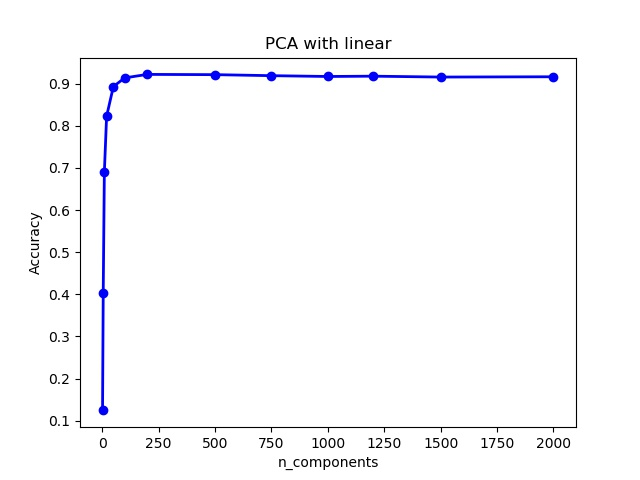
\includegraphics[width=3.75cm]{figure/PCA_linear.jpg}
%\caption{fig1}
}
\quad
\subfigure[metric Mean Rank comparison on dataset AceKG]{
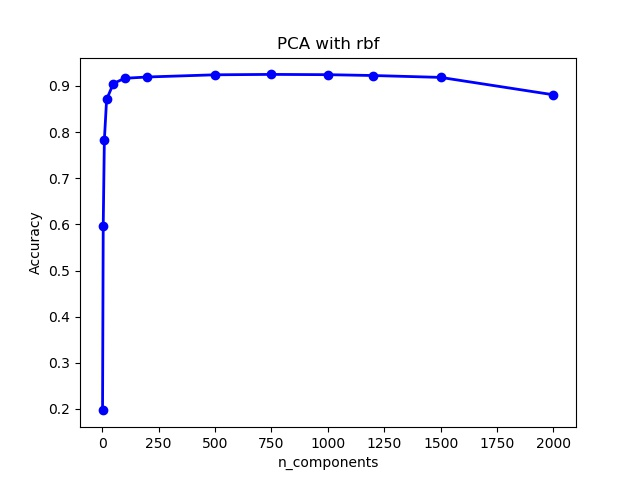
\includegraphics[width=3.75cm]{figure/PCA_rbf.jpg}
}
\caption{Mean Rank and Hits}
\label{Fig1}
\end{figure}

\subsubsection{LDA}
TODO: Qilin Chen\\

\subsection{Feature Learning}
\subsubsection{t-SNE}
TODO: Qilin Chen\\
\subsubsection{LLE}
TODO: Qilin Chen\\
\subsubsection{AutoEncoder}
TODO: Qilin Chen\\

\section{Conclusion}
TODO: Qilin Chen\\
\section*{Acknowledgement}

\bibliography{bibfile.bib}
\end{document}